%----------------------------------------
% Write your notes here
%----------------------------------------

\section{Introduction}
This lecture is a continuation from the last one. Last class, we went through the first three questions of "how one should evaluate research results", 
\begin{itemize}
  \item Was the research done and reported honestly / correctly?
  \item Is the result "real" or an artifact of the data / analysis?
  \item Will it hold up over time?
  \item How robust is the result to small changes?
  \item How important / useful is the finding?
\end{itemize}
And this class, we will keep exploring these questions through:
\begin{itemize}
    \item Common misunderstandings of $\alpha$
    \item Effect size 
    \item P-hacking
\end{itemize}



\section{Reminder of definitions from last class}
\begin{itemize}
    \item Honesty
    \begin{itemize}
        \item Was the data accurately collected and reported?
    \end{itemize}
    \item Reproducibility
    \begin{itemize}
        \item Can you independently verify the exact results using the \textbf{same data} and the \textbf{same analysis}?
    \end{itemize}
    \item Replicability
    \begin{itemize}
        \item Will the result hold up with \textbf{new data} but the \textbf{same analysis}?
    \end{itemize}
\end{itemize}


\section{Quiz---Clarifying common misunderstandings of $\alpha$}
\begin{itemize}
    \item Question:
    \begin{itemize}
        \item You do 1,000 experiments for 1,000 different research questions
        \item Only 30\% of these experiments investigate real effects
        \item You set your significance level $\alpha$ to 5\%
        \item You use a small sample size such that your power 1 - $\beta$ 35\%
        \item Given that one of these experiments shows statistical significance, what's the probability that it's a real effect?
    \end{itemize}
    \item Solution:
    \begin{itemize}
        \item Standard (yet confusing) way---Bayes rule
        \item Easier way---Draw a tree\\
        \begin{figure}[ht!]
            \begin{center}
                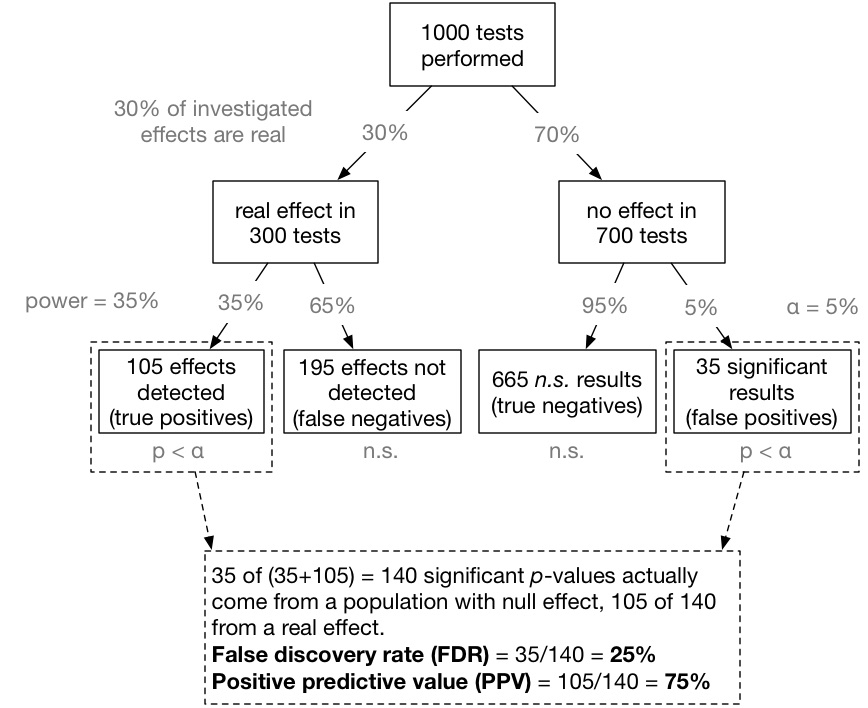
\includegraphics[width=0.7\textwidth]{figures/PPV_tree.jpeg}
                \caption{
                Tree diagram for this quiz}
                \label{fig:tree_diagram}
            \end{center}
        \end{figure}
        \begin{itemize}
            \item The answer we need is the 75\%.
        \end{itemize}
    \end{itemize}
    \item Explanation \& typical confusion:
    \begin{itemize}
        \item \textbf{False positive rate:} $\alpha$ = P(show significance $|$ no effect) = \textit{5\% in this problem}
        \item \textbf{True positive rate:} $1 - \beta$ (power) = P (show significance $|$ real effect) = \textit{35\% in this problem}
        \item \textbf{False discovery rate:}  P(no effect $|$ show significance) = \textit{25\% in this problem}
        \item Now, many people think that alpha means that 95\% (a.k.a 1 - $\alpha$) of the time we detect the real effect, \textbf{but 1 - $\pmb{\alpha}$ does not mean that}. 
        \begin{itemize}
            \item Given the definition of \textbf{false positive rate}, we see that only \textbf{75\%} of the time we detect the real effect (very small compared to the 95\% we thought)
            \item To make it better---up the power or down the alpha (power of 35\% is stupid--should be at least more than 50\%, otherwise we might as well flip a coin and save our time)
        \end{itemize}
    \end{itemize}
\end{itemize}

\section{Effect size--how big is that effect?}
\begin{itemize}
    \item definition on Wikipedia: a quantitative measure of the magnitude of a phenomenon
    \item \textbf{Cohen's d}
    \begin{itemize}
        \item Imagine you have two distributions
        \item The effect could be measured by only the \textit{difference between the mean} of the placebo group and experiment group
        \item However, if we want to take into account \textit{variance}:
        \begin{itemize}
            \item \textbf{Cohen'd} = {\huge $\pmb{\frac{\mu_1 - \mu_2}{\sigma}}$}
            \item $\pmb{\mu_2\, , \mu_2}$ are the means of the 2 distributions
            \item $\pmb{\sigma}$ the same (pooled) standard deviation of both groups
        \end{itemize}
    \end{itemize}
    \item Implications
    \begin{itemize}
        \item In real world, when we apply testing to a very big population, we can potentially have a very small distance in mean (very commonly around or below 0.2). However, since we have a big population, the variance is very small. Therefore the effect size can be big. 
        \item The fact that I reject the null does not tell me how big a difference the means are
        \item Related term: AUC, the probability of superiority P(treatment > control)
    \end{itemize}
\end{itemize}

\section{P-hacking---what happens when we get fooled by randomness}
\begin{itemize}
    \item Read \href{https://journals.sagepub.com/doi/10.1177/0956797611417632}{this paper} that discusses these studies and talk about the danger of p-hacking
    \item Study 1 (music from a time with high age contrast make people feel older)
    \item Study 2 (music from a time with high age contrast make people actually older)
    \item The problem with this study at first glance:
    \begin{itemize}
        \item father's age is a weird and unreliable measurement
        \item songs are different from one study to another
        \item the sample size is too small (20)
    \end{itemize}
    \item What they actually did:
    \begin{itemize}
        \item they had 34 students in the sample, but they threw out a bunch when analyzing 
        \item they only had three songs
    \end{itemize}
    \item What is wrong with it:
    \begin{itemize}
        \item When doing exploratory data analysis and something shows up, and they decided it’s interesting immediately 
        \item they are doing selective overfitting
        \item tested after every 10 students surveyed, and stopped surveying when found significance
        \item Eventually, if you ask enough questions about the data--then you are gonna get significance with some question
    \end{itemize}
    \item So how do we know that we are not fooling ourselves:
    \begin{itemize}
        \item tell the difference between \textbf{confirmatory analysis} and textbf{exploratory data analysis}
        \item when we write our paper, need to disclose everything that we did in the experiment 
        \item do not select and report
    \end{itemize}
    \item A \href{https://aspredicted.org/}{site} that helps with study before you go into it:
    \begin{itemize}
        \item they have couple check mark questions
        \item Last question: are the data for the study ready? If the answer is yes, then not good. (experiment vs. observation)
    \end{itemize}
\end{itemize}

\section{Predicting employee satisfaction in Microsoft---Jake's "failed?" study}
\begin{itemize}
    \item Take a look at \href{https://www.nytimes.com/2019/02/15/opinion/sunday/email-etiquette.html}{this article} and \href{https://medium.com/@duncanjwatts/the-organizational-spectroscope-7f9f239a897c}{the study at Microsoft} that the author discussed.
    \item So what happened? 
    \begin{itemize}
        \item Data: all the emails, and a survey to all employees
        \item Method:Random forest and logistic models
        \item Predict: people would be happy with work-life balance
        \item Result: Good results--good prediction
        \item However, after a year, when they did a \textbf{pre-registering predictive models}
        \begin{itemize}
            \item they pre-wrote the exact process and question they want to explore
            \item they used the exact same survey result, but with email data updated
            \item It failed quite badly, using the same method
            \item why: the way people use email has completely changed over a year
        \end{itemize}
    \end{itemize}
    \item what can we learn from this?
    \begin{itemize}
        \item It is important to do a pre-registering predictive models
        \item So we do not just fall into trap of testing a bunch of hypothesis until one works
        \item And it force you to think hard on what exactly you wanted
        \item It avoids p-hacking
        \item And this is what people should be doing
    \end{itemize}
\end{itemize}


\section{How to do R-markdown and makefile}

R-markdown is similar to jupyter notebook. You can export a pdf or html from a structured block format r code.\\
Makefile allows you to organize all the files needed to run your code and produce the result. It has dependencies of your files clearly laid out, and makes everyone's life easier.\\
If you want to check out the template Jake gives. See the \href{https://github.com/jhofman/msd2019/blob/master/lectures/lecture_6/writeup.Rmd}{R markdown write up} and \href{https://github.com/jhofman/msd2019/blob/master/lectures/lecture_6/Makefile}{makefile write up}in git-hub.


\section{Homework 2 explanation (if needed)}

\begin{itemize}
  \item Problem 1
  \begin{itemize}
      \item should be a one-line solution with r code
  \end{itemize}
  \item Problem 2
  \begin{itemize}
      \item do them on the markdown file
      \item Problems are from bit by bit book
  \end{itemize}
  \item Problem 3 
  \begin{itemize}
      \item we are forgetting the past faster and faster
      \item Take the string 1883 and each year after that, measure the frequency of the appearance of the word compare to all other words
      \item $Freq =  \frac{num times\, 1883\, appeared\, in\, some\, year}{total \,num\, words\, printed\, in\, that\, year}$
      \item Small plots: compare the half life of the words over all years (the bottom graph only showed 3 years)
      \item Tool: Google books ngram viewer
      \item Data: need to get it from the website, compresses, confusing, weird format, many extra data, super big file size (but most do not match what we need)
      \item Only use the ones start with “1” in one-gram, instruction on github, and use shell to process the data first--use the fancy egrep stuff to clean (make sure we do not match 195743, but only 1957)
      \item One line solution for all shell stuff 
      \item Submit all through github
  \end{itemize}
\end{itemize}
